\section{Inverse Kinematics}
Recap forward kinematics: Given a joint configuration, find the pose of some part of the robot.\\
Inverse kinematics: Given a pose, figure out the joint configurations.

Input data for the problem is of the form:
\[ T=\left[\begin{array}{cc}
R & t \\
0 \; 0 \; 0 & 1
\end{array}\right] \]
This is a nonlinear problem, thus it's not sure if there is a (unique/multiple/infinite/outside-of-workspace/none) solution. Inverse kinematics are not explicitly discussed the Stanford lecture and there is not particular exercise on it (albeit it is included in the lecture). 

\subsection{Multiplicity of Solutions}
If there are multiple solutions (configurations), choose the closest one:

{\centering 
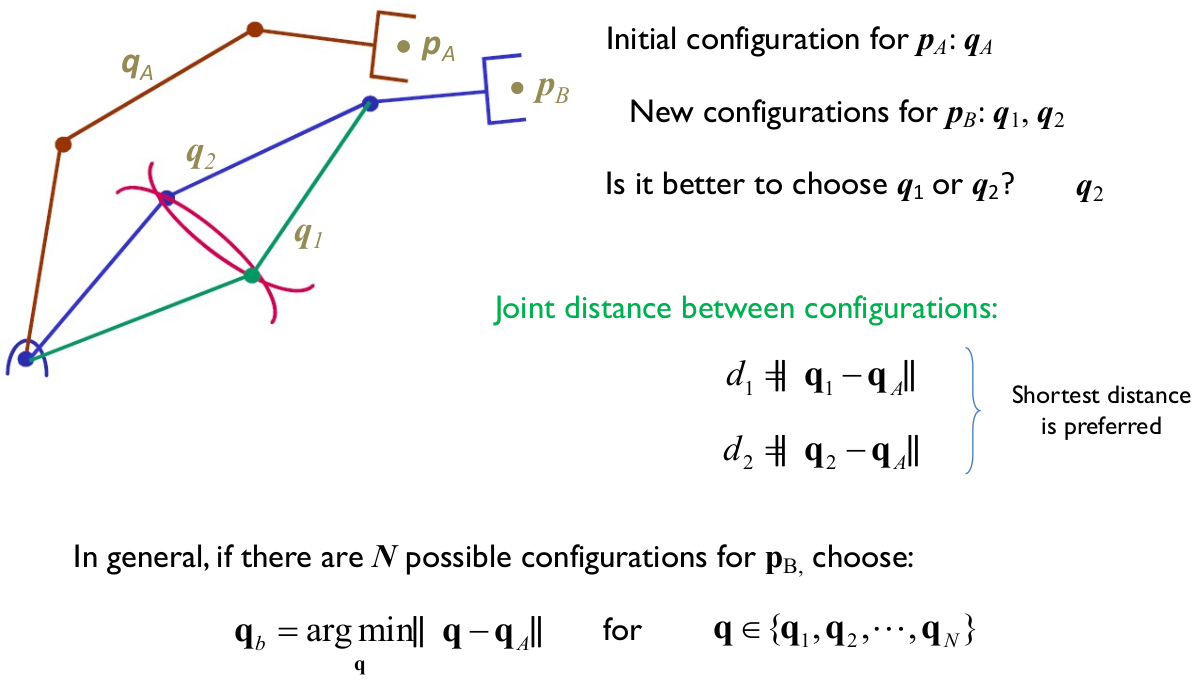
\includegraphics[width=13cm]{sections/imgs/12.png}
\\}
\subsubsection{Redundancy}
{\centering 
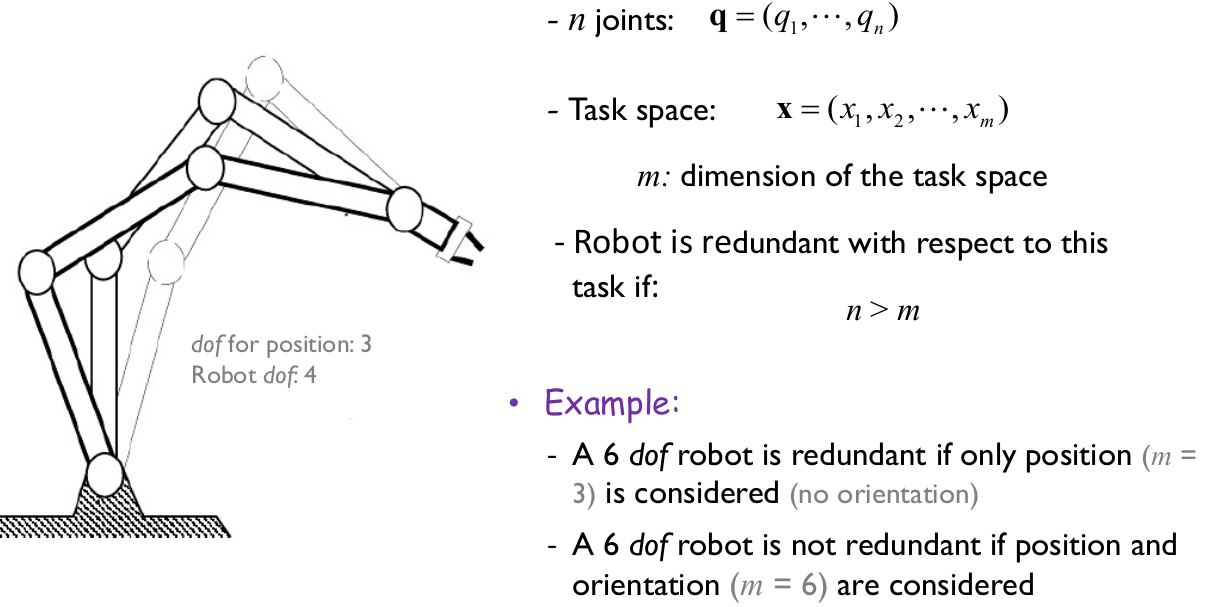
\includegraphics[width=13cm]{sections/imgs/13.png}
\\}

\subsection{Analytic solutions for the inverse kinematics}
\subsubsection{Geometric solution}
\begin{itemize}
	\item only when robot has 3 or less dofs
	\item not a generic solution
\end{itemize}

{\centering 
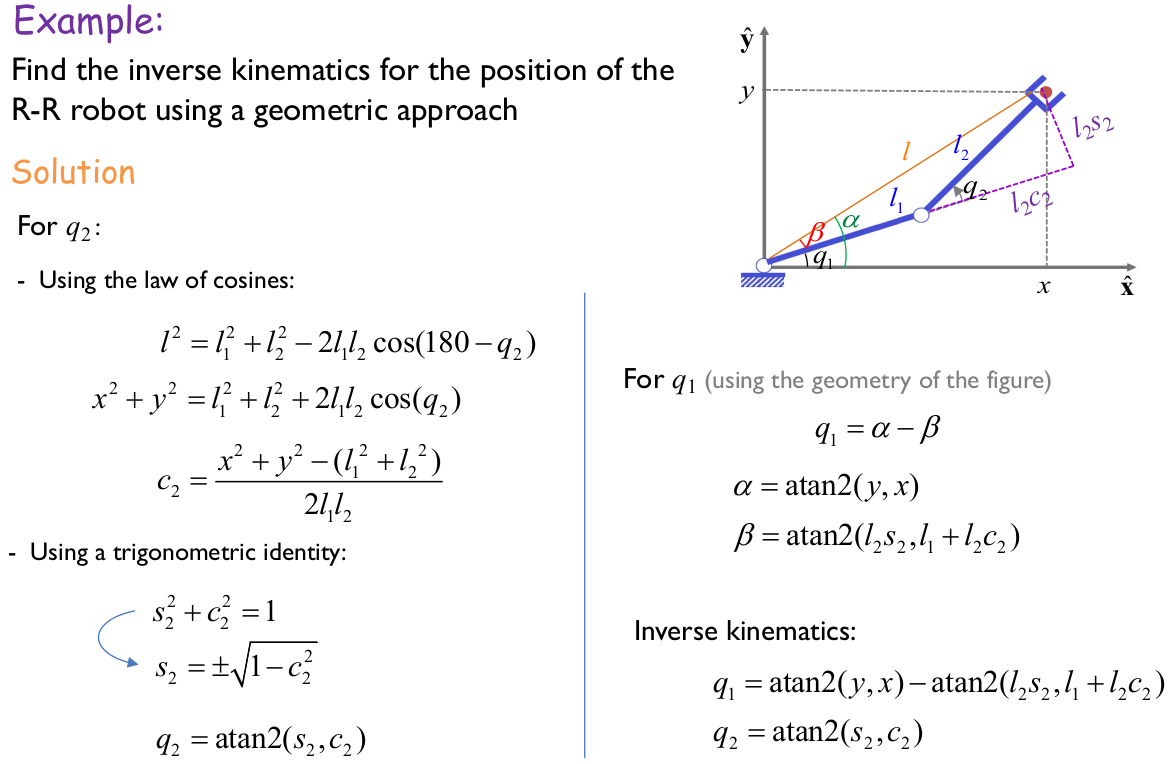
\includegraphics[width=15cm]{sections/imgs/14.png}
\\}

\subsubsection{Algebraic solution}
Solution using algebraic (and polynomial) equations.\\
Given: Formula to find the kinematic equations of an arm easily, given link params. E.g.:

{\centering 
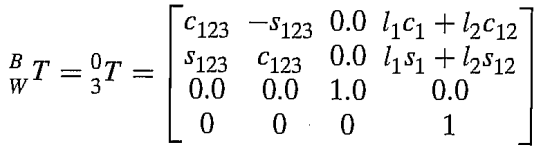
\includegraphics[width=6cm]{sections/imgs/15.png}
\\}

This describes the wrist (manipulator) frame relative to the base frame.\\
We also know what is necessary to describe such a position/orientation:

{\centering 
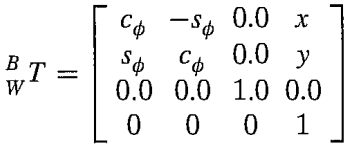
\includegraphics[width=4cm]{sections/imgs/16.png}i
\\}

So just an x-y positon and an angle \(\phi\).
By equating both, we get a set of nonlinear equations, which have to be solved for $ l_1 , l_{2} , \theta $, using magical algebra:

{\centering 
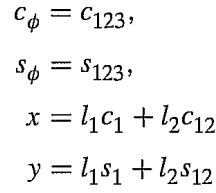
\includegraphics[width=3cm]{sections/imgs/17.png}
\\}

\subsubsection{Example}

\begin{center}
	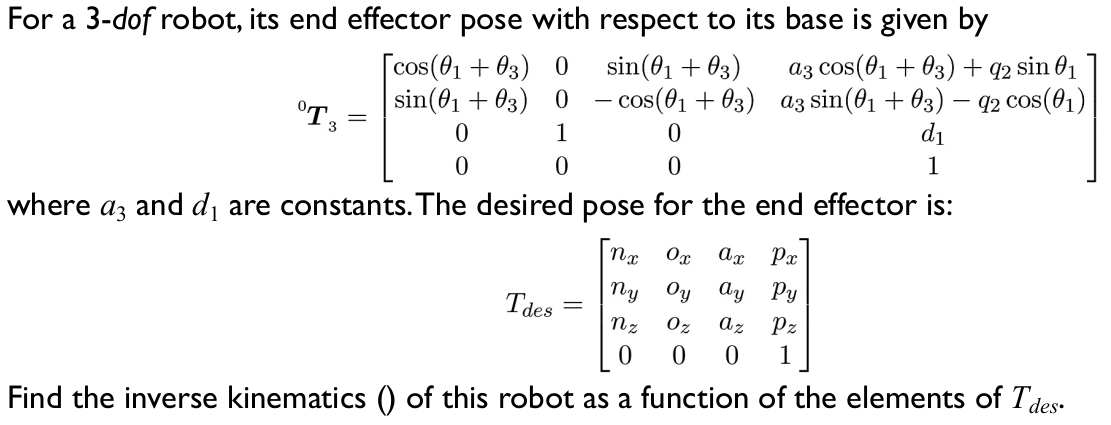
\includegraphics[width=8cm]{sections/imgs/18.png}\\
	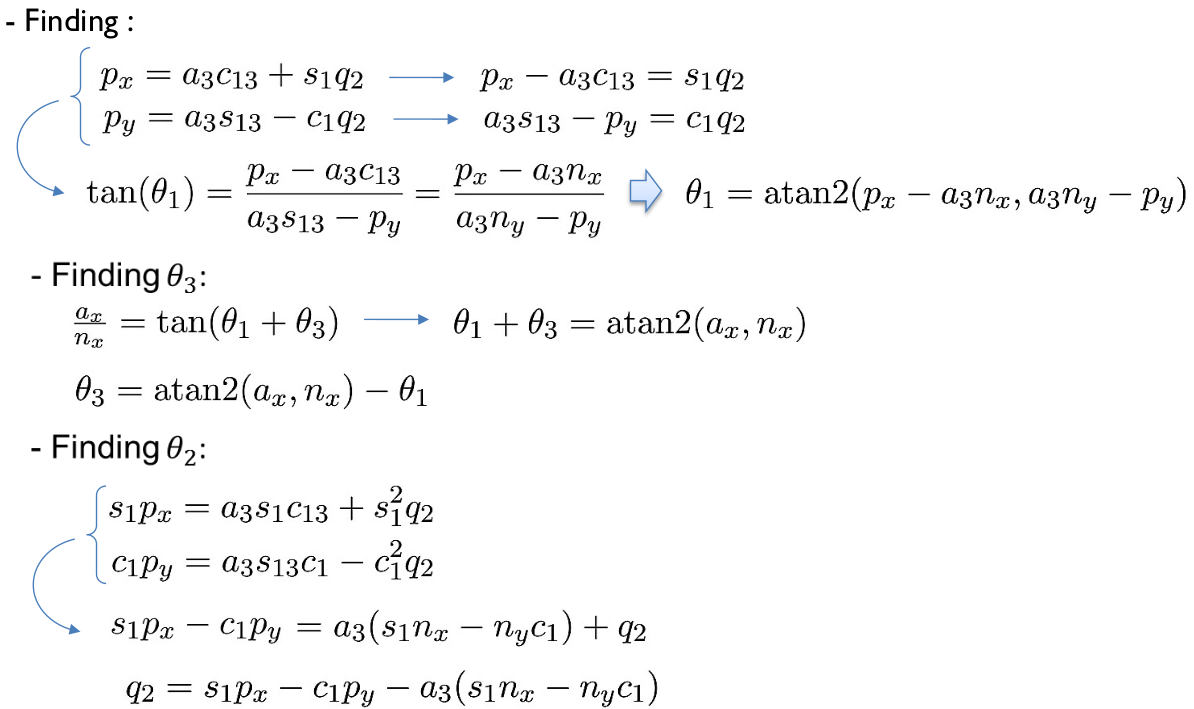
\includegraphics[width=9cm]{sections/imgs/19.png}
\end{center}

\subsection{Numeric solutions to the inverse kinematics}
Mainly used when..
\begin{itemize}
	\item no analytic solution
	\item $ \infty $ solutions
	\item too difficult to find a solution
\end{itemize}
{\centering 
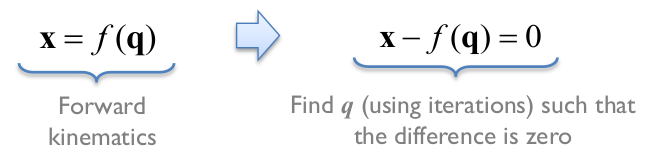
\includegraphics[width=8cm]{sections/imgs/20.png}
\\}
Uses the Jacobian matrix:
\[J (q) = \frac{\partial f (q)}{\partial q} \quad J (q) \in \mathcal{R}^{n \times m}  \]
Where $ n $ is the size of $ q $ (number of joints) and $ m $ is the size of $ x $ (size of task space)

\subsubsection{Newton's Method}

\begin{center}
	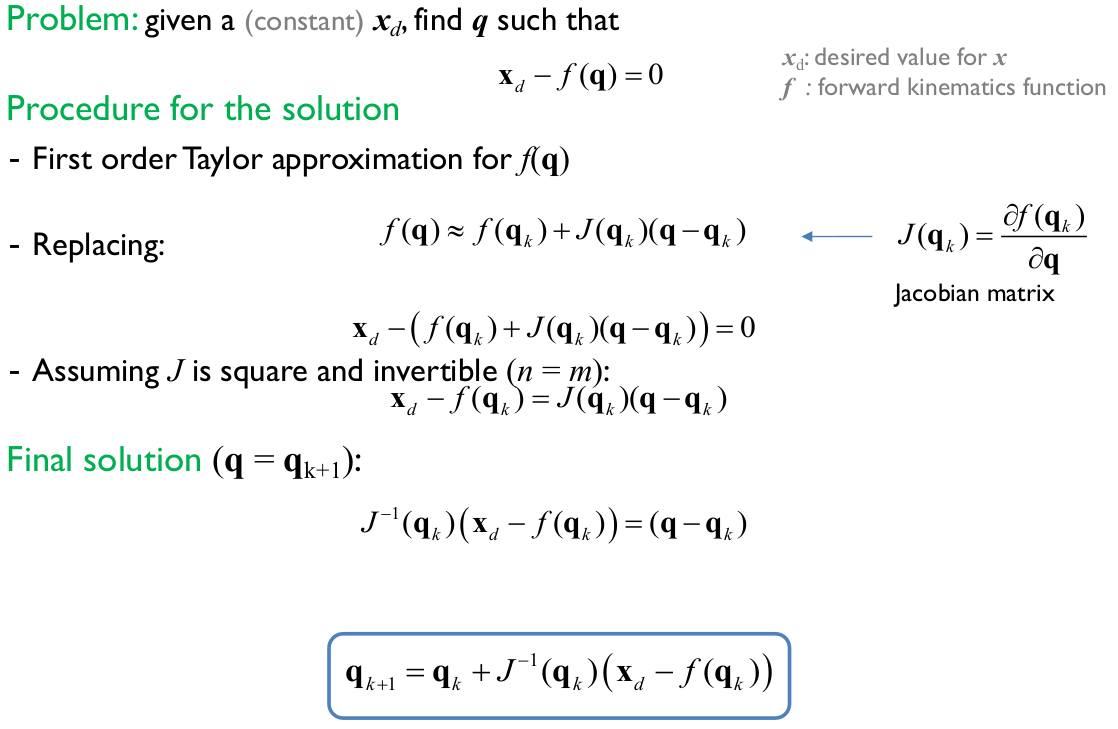
\includegraphics[width=11cm]{sections/imgs/21.png}\\
	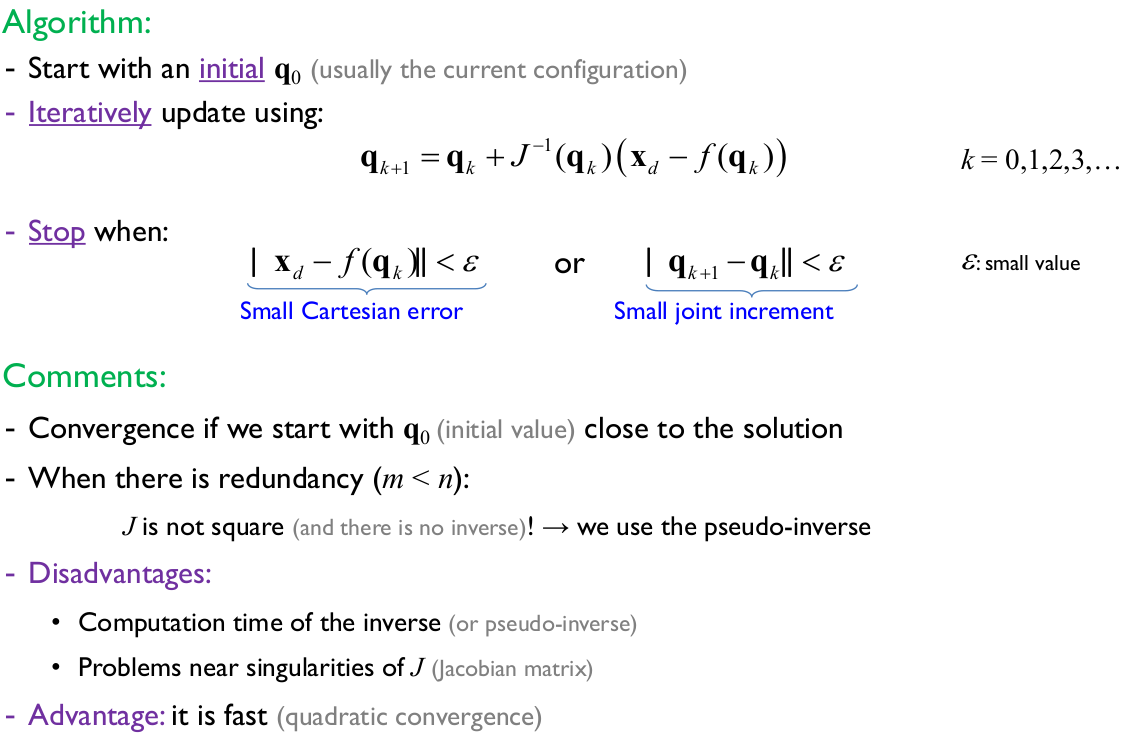
\includegraphics[width=11.4cm]{sections/imgs/22.png}
\end{center}
Example in slides.

\subsubsection{Gradient Descent Method}
\begin{center}
	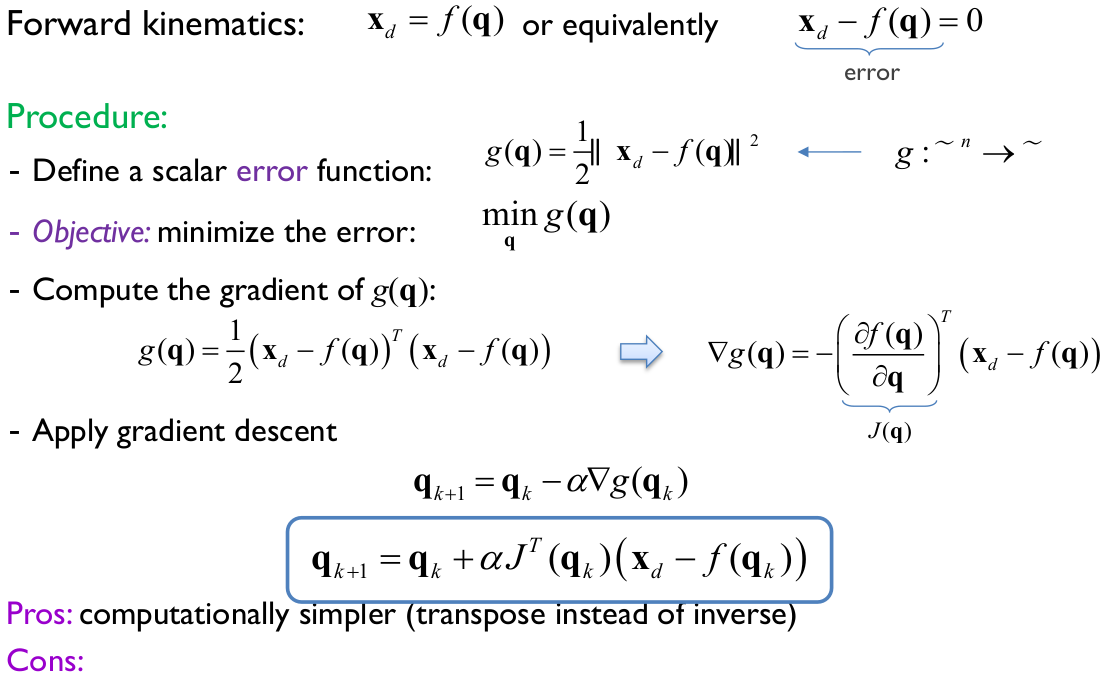
\includegraphics[width=11cm]{sections/imgs/23.png}
\end{center}
Example in slides.

\subsection{Numeric computation of the Jacobian}
For complex robots it is tedious to compute the Jacobian numerically.\\
\textbf{Solution:} Numeric differentiation

\begin{center}
	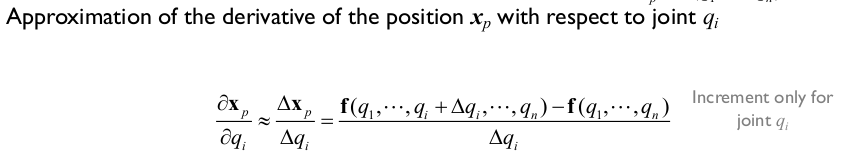
\includegraphics[width=12cm]{sections/imgs/24.png}\\
	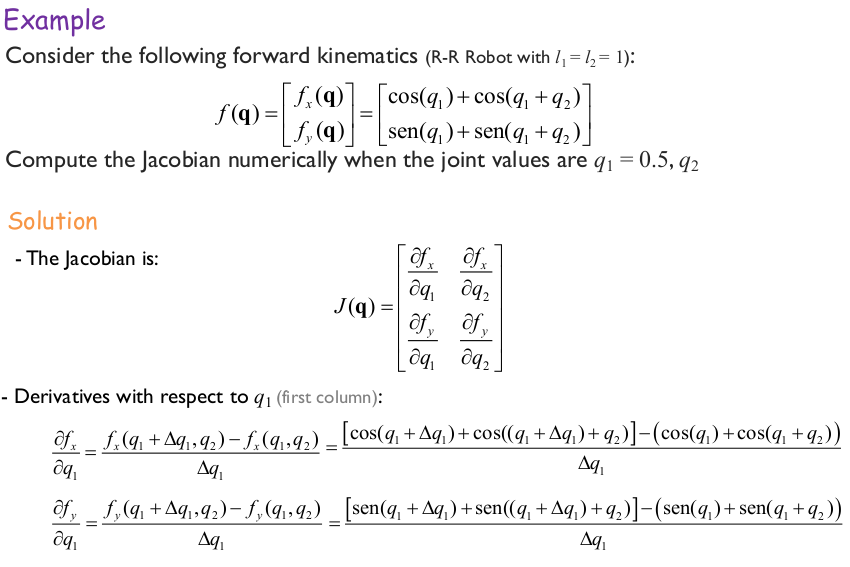
\includegraphics[width=12cm]{sections/imgs/25.png}\\
	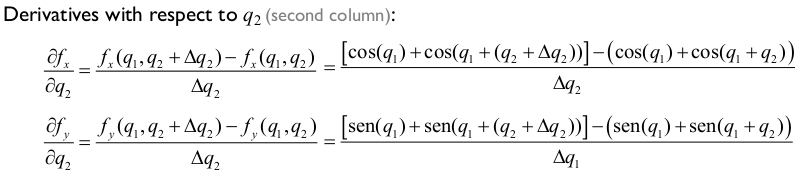
\includegraphics[width=12cm]{sections/imgs/26.png}\\
	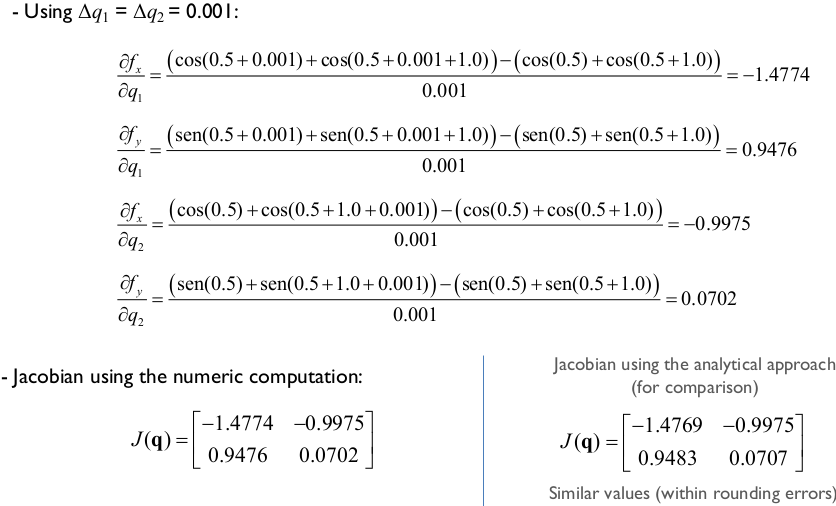
\includegraphics[width=12cm]{sections/imgs/28.png}	
\end{center}

